

\chapter{Modelling Indoor Human Location Behaviour }
\label{chapter:Human location}
Domestic service robots in future should be able to gather knowledge about all the locations in the home, the user likes to hang around. Additionally they should also know the time period when the users occupy their favourite places. This acquired knowledge of the human location behaviour shall enable the robots to make informed decisions for completing their tasks. For example what time to clean a particular room based  on least unoccupied time period or when to turn on the heater of the room. 

In this chapter we focus on this knowledge accession of users location behaviour based on spatio-temporal observations made by the robot. The advancement in long term autonomous navigation \cite{krajnik_life-long_2015} and the rapid adoption of databases in the robots \cite{niemueller2012generic}, has made the information collection for such knowledge generation possible in service robots. However even with these advancements there are some challenges which still needs to be addressed.  In more details, these challenges are the (i) modelling human location behvioud (ii) prediction of future location (iii) learning all these with sparse observations made by the robots. 

Significant progress has been made the problem by researchers in the field of human location behaviour, which is to learn the patterns in human location outdoors. Approaches for learning routine mobility  range from purely temporal (\cite{mcinerney2013modelling, scellato2011nextplace}), spatial (\cite{gao2012exploring,song2006evaluating}), to a combination  of  both  (\cite{eagle2009eigenbehaviors}). Non-parametric Bayesian methods are also gaining popularity given their ability to refine models as more data arrives. Chen et al. (2012) used a Gaussian process to model congestion on road networks, while Gao et al. (2012) used a hierarchical Pitman Yor process to model check-in behaviour on location-based social networks. Indoor human location behaviour was studied by \cite{krajnik_wheres_2015} using Fourier transform methods and Gaussian mixture models. 

While \cite{krajnik_wheres_2015}  work is first step towards learning human mobility behaviour in indoor environments, it failed to address the challenge of sparse dataset in domestic robots. As we have discussed earlier the observations on which the knowledge has to be learned, are sparse. We aim to demonstrate in this chapter that, by using Bayesian models, we can capture the human behaviour patterns in a sparse dataset.

We build Bayesian models which incorporate explicit domain knowledge and the structural knowledge about our data. Human behaviours are periodic in nature with a daily cycle. The models developed use this domain knowledge to extract the patterns emerging from the data caused by periodicity.

\section{Dirichlet Categorical model }

Dirichlet Categorical model (DCM) is a two-level Bayesian model. The basic idea is that observations of each time period is characterized by a distribution over the possible locations.

The data are the observed human location $x_{ij}$ for $i = 1 \dots T$ time periods and then $j = 1, \dots , N$  are the observations.  We assume that the latent pattern in the persons location per period are distributed as a categorical distribution. The number of periods $T$ for our model is fixed to 24 corresponding to the number of hours in a day. 

The Dirichlet-Categorical model is the generalization of the Beta-Binomial model to multiple classes of a categorical or multinomial distribution. The conjugate prior for the categorical distribution is the Dirichlet distribution. The model estimates the posterior distribution of $\theta_i$ given our current data and prior beliefs. Our prior beliefs are encoded in the model through the hyper-parameter $\alpha$, which represents pseudo-counts of what we believe the data should look like – typically set as 1's for weak uniform beliefs. The probabilistic graphical model of  DCM is shown in Figure~\ref{dcm}

\noindent
\begin{figure}[htp]

\begin{minipage}{0.3\textwidth}
\centering

\tikz {
\node [const]                  (alpha) {$\alpha$};
\node [below=of alpha, latent]  (theta) {$\theta_i$};
\node [below=of theta, obs]     (x)     {$x_{ij}$};
\edge {alpha} {theta};
\edge {theta} {x};
\plate {trials} {(x)} {j location};
\plate {bags} {(theta)(x)(trials)} {i time};
}

\end{minipage}%
\begin{minipage}{0.7\textwidth}

\begin{equation*}
	\alpha = <1, 1, .... , 1 > 
\end{equation*}
\begin{equation*}
	\theta_i  \sim Dirichlet(\alpha)
\end{equation*}
\begin{equation*}
	x_{ij} \sim Categorical(\theta_i)
\end{equation*}
\end{minipage}
\caption[Dirichlet categorical graphical model representation]{Graphical model representation of DCM. The boxes are ``plates" representing replicates. The outer plates represents hours of a day, while the inner plate represents the choice of locations within each hour.}
\label{dcm}
\end{figure}

With the graphical model, the dependencies among the many variables can be captured concisely. The boxes are ``plates” representing replicates. The outer plate represents the hours of the day, while the inner plate represents the repeated choice of locations within each hour. Thus:

	$\alpha$ is  parameter of the dirichlet prior on per-period location distribution, 
	
	$\theta_i$ is the location distribution for period $i$  ,
	
	$x_{ij}$ is the observed location of the person in period $i$.
	
The $ x_{ij}$ are the only observable variables, and the other variables are latent variables. 

\section{Hierarchical Dirichlet Categorical Model}
\label{sec: HDCM}

Observations made only by a domestic robot using internal sensors and not using any external sensors creates the serious problem of sparsity. There are very much likely that some time periods there will be no observations available to learn. Maximum likelihood estimates of the categorical parameters assign uniform probability to the locations in these time periods. The standard approach to coping with this problem is to sharing statistical strength between time periods: it is as if the location we observe for each time period also provides weaker indirect location relevant to other time periods. In machine learning and statistical science this phenomenon is often called \emph{learning to learn} or \emph{transfer learning}. Intuitively, knowing something about the location of person in the 9'o clock can help in gaining some information at 10'o clock. 

By placing a Dirichlet hyper-prior on the several Dirichlet parameter we obtain a hierarchical model. The hyper-prior makes it possible for sharing the learned knowledge from one prior to another. Thus learning about the location pattern at a higher level of abstraction helps to share it with the lower levels which have no observations.

The probabilistic graphical model of  hierarchical model is shown in Figure \cite{hdcm}

\noindent
\begin{figure}[htp]

\begin{minipage}{0.3\textwidth}
\centering

\tikz {
\node [const]                   (alpha) {$\alpha$};
\node [below=of alpha, latent]  (beta)  {$\beta$};
\node [below=of beta, latent]   (theta) {$\theta_i$};
\node [below=of theta, obs]     (x)     {$x_{ij}$};
\edge {alpha} {beta};
\edge {beta} {theta};
\edge {theta} {x};
\plate {trials} {(x)} {j location};
\plate {bags} {(theta)(x)(trials)} {i time};
}

\end{minipage}%
\begin{minipage}{0.7\textwidth}

\begin{equation*}
	\alpha = <1, 1, .... , 1 > 
\end{equation*}
\begin{equation*}
	\beta \sim Dirichlet(\alpha)
\end{equation*}
\begin{equation*}
	\theta_i  \sim Dirichlet(\beta)
\end{equation*}
\begin{equation*}
	x_{ij} \sim Categorical(\theta_i)
\end{equation*}
\end{minipage}
\caption[Hierarchical dirichlet categorical graphical model representation]{Hierarchical Dirichlet Categorical Model. The boxes are ``plates" representing replicates. The outer plates represents hours of a day, while the inner plate represents the choice of locations within each hour.}
\label{hdcm}
\end{figure}

The model can be explained as:

	\boldmath{$\alpha$} is  constant dirichlet prior for the hyperprior, 
	
	$\beta$ is a Dirichlet hyperprior,
	
	$\theta_i$ is the location distribution for period $i$  ,
	
	$x_{ij}$ is the observed location of the person in period $i$.
	
Thus we have categorical variables dependent on multiple priors sharing a hyperprior.


\section{Aruba Dataset}
In our thesis, we have used a  publicly-available  dataset Aruba, published by the Lincoln Center for Autonomous Systems(LCAS). The dataset is of a person's location in a home collected at a smart apartment by \cite{aruba} from the Center for Advanced Studies in Adaptive Systems, CASAS .

The testbed where the dataset was collected is a  three-bedroom apartment located on the Washington State University that is part of CASAS smart home project. 
\begin{figure}[htp]
\centering
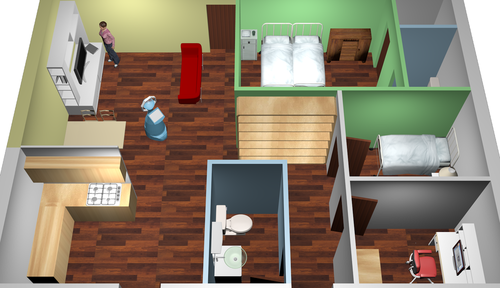
\includegraphics[width=\textwidth]{images/aruba-flat.png}
\caption{Aruba apartment visualization}
\label{aruba}
\end{figure}
As shown in Figure~\ref{aruba}, the smart apartment test bed includes three bedrooms, one bathroom, a kitchen, and a living / dining room.  The apartment is equipped with motion sensors distributed approximately 1 meter apart throughout the space. The Aruba dataset was extracted from these motion sensor dataset provided by CASAS. The dataset contains the location of a person in the apartment every minute for 16 weeks.


We visualize the dataset as a heatmap over locations distributed over different periods. As explained in chapter~\ref{sec:Problem formulation}, we try to learn daily patterns by dividing the observations into per hour periods. As we can see there are some prominent patterns present which can be learned. For example the usage of the bedroom, living room, outside and kitchen.

\begin{figure}[htp]
\centering
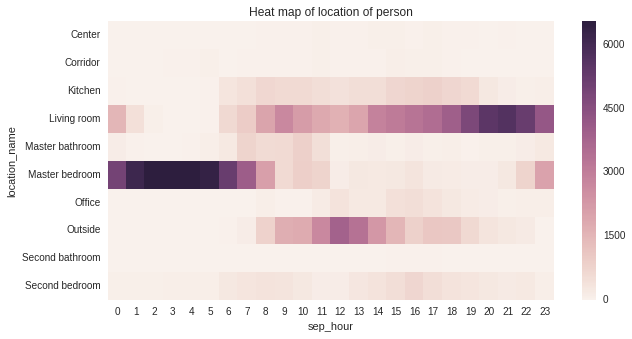
\includegraphics[width=\textwidth]{images/aruba-data.png}
\caption[Aruba dataset heatmap]{Aruba dataset heatmap : The x-axis are the locations of the home, y-axis are the hours of the day. The intensity of the color in each box indicates the number of times the person is present in that location. Higher the intensity means more time is spent by the person in that location at that time.}
\label{aruba-visual}
\end{figure}

A histogram visualization of the observations over different location in the home is show in Figure~\ref{aruba-hist}

\begin{figure}[htp]
\centering
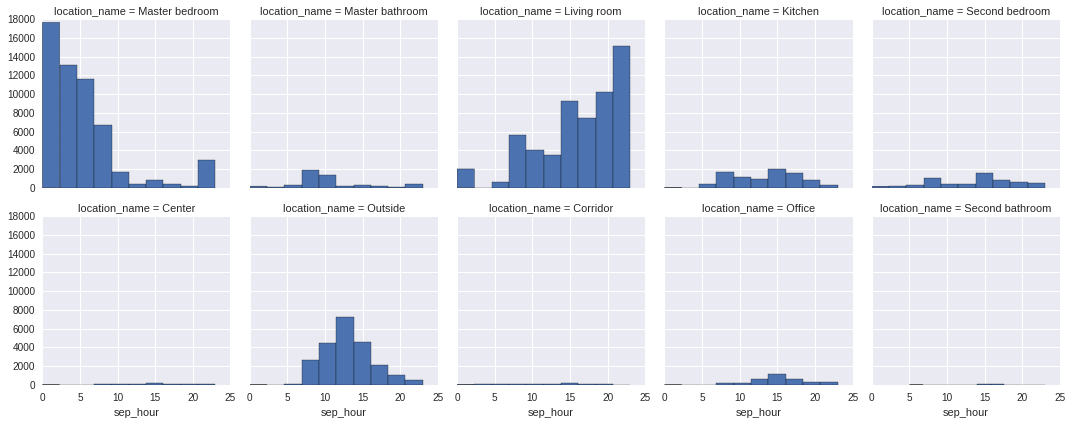
\includegraphics[width=\textwidth]{images/aruba-hist.png}
\caption[Aruba dataset histogram]{Aruba Dataset Histogram : Each box corresponds to histogram of each locations. The x - axis represents the time of the day(0-24) }
\label{aruba-hist}
\end{figure}


\subsection*{Sparsification}
Aruba dataset is a large dataset as compared to an person location dataset we assume the robot will be able to generate. The Aruba dataset has recordings of every minute for 118 days, which is 161280 readings.
On the contrary the assumed dataset which will be collected by the robot by autonomously roaming in a home will be just 3-5 readings per day.
So for simulating the sparsity in the object location dataset we will sparsify the ARUBA dataset by random selecting only selecting 3-5 readings each day.

After sparsification by randomly selecting 5 readings per day the dataset is reduced to 590 observations. The heatmap the of the sparsified dataset is shown in Figure~\ref{aruba-reduced-hist}. 

\begin{figure}[htp]
\centering
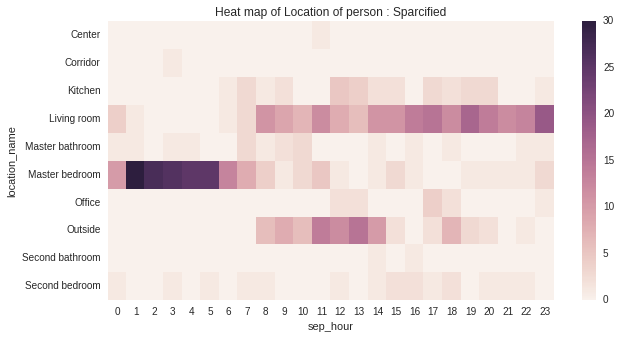
\includegraphics[width=\textwidth]{images/aruba-reduced-heatmap.png}
\caption[Aruba sparcified dataset heatmap]{Aruba sparcified dataset heatmap :The x-axis are the locations of the home, y-axis are the hours of the day. Compared to the complete observations the sparcified data set the patterns are not distinct}
\label{aruba-reduced-hist}
\end{figure}

\FloatBarrier

\section{Evaluation}
\todo[inline]{TODO}
In these experiments, we estimated the parameters of the DCM using the sparsified observations. We then trained a support vector machine(SVM) and Random Forest on the same sparsified observations. Then compared the results of SVM, Random forest, DCM and HDCM by cross validation.



\missingfigure{Cross validation results}

The models were also compared with the models developed by \cite{krajnik_wheres_2015}  based on the average time required by the robot to locate the user in the home.

\missingfigure{Timing results}




\section{Discussions}
\todo[inline]{
http://andrewgelman.com/2016/08/22/bayesian-inference-completely-solves-the-multiple-comparisons-problem/
http://andrewgelman.com/2013/11/21/hidden-dangers-noninformative-priors/

The point of the story in that slide is that flat priors consistently give bad inferences. Or, to put it another way, the routine use of flat priors results in poor frequency properties in realistic settings where studies are noisy and effect sizes are small.}


todo[inline]{

Why cross validation problem with SVM and probabilistic models \\
http://andrewgelman.com/2016/01/30/evaluating-models-with-predictive-accuracy/

}

In chapter \ref{chapter: object} the models captured knowledge about each location separately, while in this chapter the models can capture knowledge about multiple locations can be captured in a single model.

% section  (end)





